%!TEX encoding = UTF-8 Unicode
\documentclass[french, a4paper, 10pt, twocolumn, landscape]{article}



%% Langue et compilation

\usepackage[utf8]{inputenc}
\usepackage[T1]{fontenc}
\usepackage[french]{babel}
\usepackage{lmodern}       % permet d'avoir certains "fonts" de bonne qualite
\renewcommand{\familydefault}{\sfdefault}
%% LISTE DES PACKAGES

\usepackage{mathtools}     % package de base pour les maths
\usepackage{amsmath}       % mathematical type-setting
\usepackage{amssymb}       % symbols speciaux pour les maths
\usepackage{textcomp}      % symboles speciaux pour el text
\usepackage{gensymb}       % commandes generiques \degree etc...
\usepackage{tikz}          % package graphique
\usepackage{wrapfig}       % pour entourer a cote d'une figure
\usepackage{color}         % package des couleurs
\usepackage{xcolor}        % autre package pour les couleurs
\usepackage{pgfplots}      % pacakge pour creer des graph
\usepackage{epsfig}        % permet d'inclure des graph en .eps
\usepackage{graphicx}      % arguments dans includegraphics
\usepackage{pdfpages}      % permet d'insérer des pages pdf dans le document
\usepackage{subfig}        % permet de creer des sous-figure
% \usepackage{pst-all}       % utile pour certaines figures en pstricks
\usepackage{lipsum}        % package qui permet de faire des essais
\usepackage{array}         % permet de faire des tableaux
\usepackage{multicol}      % plusieurs colonnes sur une page
\usepackage{enumitem}      % pro­vides user con­trol: enumerate, itemize and description
\usepackage{hyperref}      % permet de creer des hyperliens dans le document
\usepackage{lscape}        % permet de mettre une page en mode paysage

\usepackage{fancyhdr}      % Permet de mettre des informations en hau et en bas de page      
\usepackage[framemethod=tikz]{mdframed} % breakable frames and coloured boxes
\usepackage[top=1.8cm, bottom=1.8cm, left=1.5cm, right=1.5cm]{geometry} % donne les marges
\usepackage[font=normalsize, labelfont=bf,labelsep=endash, figurename=Figure]{caption} % permet de changer les legendes des figures
\setlength{\parskip}{0pt}%
\setlength{\parindent}{18pt}
\usepackage{lewis}
\usepackage{bohr}
\usepackage{chemfig}
\usepackage{chemist}
\usepackage{tabularx}
\usepackage{pgf-spectra} % permet de tracer des spectres lumineux des atomes et des ions
\usepackage{pgf}

\usepackage{flexisym}
\usepackage{soul}
\usepackage{ulem}
\usepackage{cancel}

\usepackage{import}
\usepackage{physics}
\usepackage[outline]{contour} % glow around text
\tikzset{every shadow/.style={opacity=1}}


%% LIBRAIRIES

\usetikzlibrary{plotmarks} % librairie pour les graphes
\usetikzlibrary{patterns}  % necessaire pour certaines choses predefinies sur tikz
\usetikzlibrary{shadows}   % ombres des encadres
\usetikzlibrary{backgrounds} % arriere plan des encadres


%% MISE EN PAGE

\pagestyle{fancy}     % Défini le style de la page

\renewcommand{\headrulewidth}{0pt}      % largeur du trait en haut de la page
\fancyhead[L]{\textbf{\textcolor{cyan}{Cours}} - Thème 4 - La Terre un astre singulier}         % info coin haut gauche
\fancyhead[R]{\textit{Première Enseignement Scientifique}}  % info coin haut droit

% % bas de la page
% \renewcommand{\footrulewidth}{0pt}      % largeur du trait en bas de la page
% \fancyfoot[L]{}  % info coin bas gauche
\fancyfoot[R]{Lycée GT Jean Guéhenno}                         % info coin bas droit


\setlength{\columnseprule}{1pt} 
\setlength{\columnsep}{30pt}



%% NOUVELLES COMMANDES 

\DeclareMathOperator{\e}{e} % permet d'ecrire l'exponentielle usuellement


\newcommand{\gap}{\vspace{0.15cm}}   % defini une commande pour sauter des lignes
\renewcommand{\vec}{\overrightarrow} % permet d'avoir une fleche qui recouvre tout le vecteur
\newcommand{\bi}{\begin{itemize}}    % begin itemize
\newcommand{\ei}{\end{itemize}}      % end itemize
\newcommand{\bc}{\begin{center}}     % begin center
\newcommand{\ec}{\end{center}}       % end center
\newcommand\opacity{1}               % opacity 
\pgfsetfillopacity{\opacity}

\newcommand*\Laplace{\mathop{}\!\mathbin\bigtriangleup} % symbole de Laplace

\frenchbsetup{StandardItemLabels=true} % je ne sais plus

\newcommand{\smallO}[1]{\ensuremath{\mathop{}\mathopen{}o\mathopen{}\left(#1\right)}} % petit o

\newcommand{\cit}{\color{blue}\cite} % permet d'avoir les citations de couleur bleues
\newcommand{\bib}{\color{black}\bibitem} % paragraphe biblio en noir et blanc
\newcommand{\bthebiblio}{\color{black} \begin{thebibliography}} % idem necessaire sinon bug a cause de la couleur
\newcommand{\ethebiblio}{\color{black} \end{thebibliography}}   % idem
%%% TIKZ


%% COULEURS 


\definecolor{definitionf}{RGB}{220,252,220}
\definecolor{definitionl}{RGB}{39,123,69}
\definecolor{definitiono}{RGB}{72,148,101}

\definecolor{propositionf}{RGB}{255,216,218}
\definecolor{propositionl}{RGB}{38,38,38}
\definecolor{propositiono}{RGB}{109,109,109}

\definecolor{theof}{RGB}{255,216,218}
\definecolor{theol}{RGB}{160,0,4}
\definecolor{theoo}{RGB}{221,65,100}

\definecolor{avertl}{RGB}{163,92,0}
\definecolor{averto}{RGB}{255,144,0}

\definecolor{histf}{RGB}{241,238,193}

\definecolor{metf}{RGB}{220,230,240}
\definecolor{metl}{RGB}{56,110,165}
\definecolor{meto}{RGB}{109,109,109}


\definecolor{remf}{RGB}{230,240,250}
\definecolor{remo}{RGB}{150,150,150}

\definecolor{exef}{RGB}{240,240,240}

\definecolor{protf}{RGB}{247,228,255}
\definecolor{protl}{RGB}{105,0,203}
\definecolor{proto}{RGB}{174,88,255}

\definecolor{grid}{RGB}{180,180,180}

\definecolor{titref}{RGB}{230,230,230}

\definecolor{vert}{RGB}{23,200,23}

\definecolor{violet}{RGB}{180,0,200}

\definecolor{copper}{RGB}{217, 144, 88}

%% Couleur des ref

\hypersetup{
	colorlinks=true,
	linkcolor=black,
	citecolor=blue,
	urlcolor=black
		   }

%% CADRES

\tikzset{every shadow/.style={opacity=1}}

\global\mdfdefinestyle{doc}{backgroundcolor=white, shadow=true, shadowcolor=propositiono, linewidth=1pt, linecolor=black, shadowsize=5pt}
\global\mdfdefinestyle{titr}{backgroundcolor=metf, shadow=true, shadowcolor=propositiono, linewidth=1pt, linecolor=black, shadowsize=5pt}
\global\mdfdefinestyle{theo}{backgroundcolor=theof, shadow=true, shadowcolor=theoo, linewidth=1pt, linecolor=theol, shadowsize=5pt}
\global\mdfdefinestyle{prop}{backgroundcolor=theof, shadow=true, shadowcolor=propositiono, linewidth=1pt, linecolor=theol, shadowsize=5pt}
\global\mdfdefinestyle{def}{backgroundcolor=definitionf, shadow=true, shadowcolor=definitiono, linewidth=1pt, linecolor=definitionl, shadowsize=5pt}
\global\mdfdefinestyle{histo}{backgroundcolor=histf, shadow=true, shadowcolor=propositiono, linewidth=1pt, linecolor=black, shadowsize=5pt}
\global\mdfdefinestyle{avert}{backgroundcolor=white, shadow=true, shadowcolor=averto, linewidth=1pt, linecolor=avertl, shadowsize=5pt}
\global\mdfdefinestyle{met}{backgroundcolor=metf, shadow=true, shadowcolor=meto, linewidth=1pt, linecolor=metl, shadowsize=5pt}
\global\mdfdefinestyle{rem}{backgroundcolor=metf, shadow=true, shadowcolor=meto, linewidth=1pt, linecolor=metf, shadowsize=5pt}
\global\mdfdefinestyle{exo}{backgroundcolor=exef, shadow=true, shadowcolor=propositiono, linewidth=1pt, linecolor=exef, shadowsize=5pt}
\global\mdfdefinestyle{not}{backgroundcolor=definitionf, shadow=true, shadowcolor=propositiono, linewidth=1pt, linecolor=black, shadowsize=5pt}
\global\mdfdefinestyle{proto}{backgroundcolor=protf, shadow=true, shadowcolor=proto, linewidth=1pt, linecolor=protl, shadowsize=5pt}

%%%%%%
\definecolor{cobalt}{rgb}{0.0, 0.28, 0.67}
\definecolor{applegreen}{rgb}{0.55, 0.71, 0.0}

\usepackage{tcolorbox}
  \tcbuselibrary{most}
  \tcbset{colback=cobalt!5!white,colframe=cobalt!75!black}



\newtcolorbox{definition}[1]{
	colback=applegreen!5!white,
  	colframe=applegreen!65!black,
	fonttitle=\bfseries,
  	title={#1}}
\newtcolorbox{Programme}[1]{
	colback=cobalt!5!white,
  	colframe=cobalt!65!black,
	fonttitle=\bfseries,
  	title={#1}} 
\newtcolorbox{Proposition}[1]{
      colback=theof,%!5!white,
        colframe=theol,%!65!black,
      fonttitle=\bfseries,
        title={#1}}  

\newtcolorbox{Exercice}[1]{
  colback=cobalt!5!white,
  colframe=cobalt!65!black,
  fonttitle=\bfseries,
  title={#1}}  

\newtcolorbox{Resultat}[1]{
	colback=theof,%!5!white,
	colframe=theoo!85!black,
  fonttitle=\bfseries,
	title={#1}} 	

  \setlength{\tabcolsep}{20pt}

  \renewcommand{\arraystretch}{1.5}
  
  \newcommand{\pisteverte}{
	\begin{flushleft}
		\begin{tikzpicture}
			\draw (0,0) -- (0,.2);
			\draw[fill = green] (0,0.4) circle (0.2);
			\node[draw] at (1.5,0.3) {Piste verte};
		\end{tikzpicture}
		\end{flushleft}
}

\newcommand{\pistebleue}{
	\begin{flushleft}
		\begin{tikzpicture}
			\draw (0,0) -- (0,.2);
			\draw[fill = blue] (0,0.4) circle (0.2);
			\node[draw] at (1.5,0.3) {Piste bleue};
		\end{tikzpicture}
		\end{flushleft}
}
\newcommand{\pistenoire}{
	\begin{flushleft}
		\begin{tikzpicture}
			\draw (0,0) -- (0,.2);
			\draw[fill = black!80] (0,0.4) circle (0.2);
			\node[draw] at (1.5,0.3) {Piste noire};
		\end{tikzpicture}
		\end{flushleft}
}
  \newcommand{\titre}[1]{
    \begin{mdframed}[style=titr, leftmargin=0pt, rightmargin=0pt, innertopmargin=8pt, innerbottommargin=8pt, innerrightmargin=10pt, innerleftmargin=10pt]
      \begin{center}
        \Large{\textbf{#1}}
      \end{center}
    \end{mdframed}
  }


  %% COMMANDE Exercice
  
  \newcommand{\exo}[3]{
    \begin{mdframed}[style=exo, leftmargin=0pt, rightmargin=0pt, innertopmargin=8pt, innerbottommargin=8pt, innerrightmargin=10pt, innerleftmargin=10pt]
  
      \noindent \textbf{Exercice #1 - #2}\medskip
  
      #3
    \end{mdframed}
  }
  
     
  \newcommand{\questions}[1]{
    \begin{mdframed}[style=exo, leftmargin=0pt, rightmargin=0pt, innertopmargin=8pt, innerbottommargin=8pt, innerrightmargin=10pt, innerleftmargin=10pt]
  
      \noindent \textbf{Questions :}\smallskip
  
      #1
    \end{mdframed}
  }
  
  \newcommand{\doc}[3]{
    \begin{mdframed}[style=doc, leftmargin=0pt, rightmargin=0pt, innertopmargin=8pt, innerbottommargin=8pt, innerrightmargin=10pt, innerleftmargin=10pt]
  
      \noindent \textbf{Document #1 - #2}\medskip
  
      #3
    \end{mdframed}
  }
\def\width{12}
\def\hauteur{5}


\usetikzlibrary{intersections}
\usetikzlibrary{decorations.markings}
\usetikzlibrary{angles,quotes} % for pic
\usetikzlibrary{calc}
\usetikzlibrary{3d}
\contourlength{1.3pt}

\tikzset{>=latex} % for LaTeX arrow head
\colorlet{myred}{red!85!black}
\colorlet{myblue}{blue!80!black}
\colorlet{mycyan}{cyan!80!black}
\colorlet{mygreen}{green!70!black}
\colorlet{myorange}{orange!90!black!80}
\colorlet{mypurple}{red!50!blue!90!black!80}
\colorlet{mydarkred}{myred!80!black}
\colorlet{mydarkblue}{myblue!80!black}
\tikzstyle{xline}=[myblue,thick]
\def\tick#1#2{\draw[thick] (#1) ++ (#2:0.1) --++ (#2-180:0.2)}
\tikzstyle{myarr}=[myblue!50,-{Latex[length=3,width=2]}]
\def\N{90}

\tikzset{
  % style to apply some styles to each segment of a path
  on each segment/.style={
    decorate,
    decoration={
      show path construction,
      moveto code={},
      lineto code={
        \path [#1]
        (\tikzinputsegmentfirst) -- (\tikzinputsegmentlast);
      },
      curveto code={
        \path [#1] (\tikzinputsegmentfirst)
        .. controls
        (\tikzinputsegmentsupporta) and (\tikzinputsegmentsupportb)
        ..
        (\tikzinputsegmentlast);
      },
      closepath code={
        \path [#1]
        (\tikzinputsegmentfirst) -- (\tikzinputsegmentlast);
      },
    },
  },
  % style to add an arrow in the middle of a path
  mid arrow/.style={postaction={decorate,decoration={
        markings,
        mark=at position .5 with {\arrow[#1]{stealth}}
      }}},
}



\usetikzlibrary{3d, shapes.multipart}

% Styles
\tikzset{>=latex} % for LaTeX arrow head
\tikzset{axis/.style={black, thick,->}}
\tikzset{vector/.style={>=stealth,->}}
\tikzset{every text node part/.style={align=center}}
\usepackage{amsmath} % for \text
 
\usetikzlibrary{decorations.pathreplacing,decorations.markings}

%% MODIFICATION DE CHAPTER  
\makeatletter
\def\@makechapterhead#1{%
  %%%%\vspace*{50\p@}% %%% removed!
  {\parindent \z@ \raggedright \normalfont
    \ifnum \c@secnumdepth >\m@ne
        \huge\bfseries \@chapapp\space \thechapter
        \par\nobreak
        \vskip 20\p@
    \fi
    \interlinepenalty\@M
    \Huge \bfseries #1\par\nobreak
    \vskip 40\p@
  }}
\def\@makeschapterhead#1{%
  %%%%%\vspace*{50\p@}% %%% removed!
  {\parindent \z@ \raggedright
    \normalfont
    \interlinepenalty\@M
    \Huge \bfseries  #1\par\nobreak
    \vskip 40\p@
  }}
  
  \newcommand{\isotope}[3]{%
     \settowidth\@tempdimb{\ensuremath{\scriptstyle#1}}%
     \settowidth\@tempdimc{\ensuremath{\scriptstyle#2}}%
     \ifnum\@tempdimb>\@tempdimc%
         \setlength{\@tempdima}{\@tempdimb}%
     \else%
         \setlength{\@tempdima}{\@tempdimc}%
     \fi%
    \begingroup%
    \ensuremath{^{\makebox[\@tempdima][r]{\ensuremath{\scriptstyle#1}}}_{\makebox[\@tempdima][r]{\ensuremath{\scriptstyle#2}}}\text{#3}}%
    \endgroup%
  }%

\makeatother


\definecolor{darkpastelgreen}{rgb}{0.01, 0.75, 0.24}
\newcommand{\mobiliser}{
  % \begin{flushleft}
    \begin{tikzpicture}[scale=0.6]
      % \draw (0,0) -- (0,.2);
      \draw[color = darkpastelgreen, fill = darkpastelgreen] (0,-0.3) circle (0.3)node[white]{M};
      % \node[draw, white] at (0,-0.3) {\textbf{M}};
    \end{tikzpicture}
    % \end{flushleft}
}

\newcommand{\realiser}{
  % \begin{flushleft}
    \begin{tikzpicture}[scale=.6]
      % \draw (0,0) -- (0,.2);
      \draw[color = blue, fill = blue] (0,-0.3) circle (0.3) node[white]{R};
      % \node[draw, white] at (0,-0.3) {\textbf{R}};
    \end{tikzpicture}
    % \end{flushleft}
}

\definecolor{bostonuniversityred}{rgb}{0.8, 0.0, 0.0}

\newcommand{\analyser}{
  % \begin{flushleft}
    \begin{tikzpicture}[scale=.6]
      % \draw (0,0) -- (0,.2);
      \draw[color = bostonuniversityred, fill = bostonuniversityred] (0,-0.3) circle (0.3) node[white]{A};
      % \node[draw, white] at (0,-0.3) {\textbf{A}};
    \end{tikzpicture}
    % \end{flushleft}
}
\definecolor{amethyst}{rgb}{0.6, 0.4, 0.8}

\newcommand{\communiquer}{
  % \begin{flushleft}
    \begin{tikzpicture}[scale=.6]
      % \draw (0,0) -- (0,.2);
      \draw[color = amethyst, fill = amethyst] (0,-0.3) circle (0.3) node[white]{C};
      % \node[draw, white] at (0,-0.3) {\textbf{C}};
    \end{tikzpicture}
    % \end{flushleft}
}

\newcommand{\applicationnumerique}{\textbf{A.N.:}}

\usepackage{esint}
\usepackage{breqn}
\usepackage{colortbl}
\newcommand{\objectifs}[1]{
	\begin{minipage}{.02\textheight}
	\rotatebox{90}{\textbf{\large Objectifs}}
	\end{minipage}
	\begin{minipage}{.9\linewidth}
			#1 
	\end{minipage}
}
%%
%%
%% DEBUT DU DOCUMENT
%%

\begin{document}

\section*{Leçon 26: Cinématique relativiste: Expérience de Michelson et Morley}
\hrulefill\\
	\underline{Niveau:}
	\begin{itemize}
		\item Licence 3
	\end{itemize}
	\underline{Pré-requis:} 
	\begin{itemize}
		\item Mécanique
		\item électromagnétisme
		\item Optique
	\end{itemize}
	\underline{Bibliographie:}
	\begin{itemize}
		\item BFR \textit{Mécanique 1}
		\item Pérez \textit{Relativité}
		\item Purcell and Morin \textit{Electricity and magnetism}
		\item \url{https://fr.wikipedia.org/wiki/Exp%C3%A9rience_de_Michelson_et_Morley}
	\end{itemize}
\hrulefill

\section*{1. Introduction: les problèmes de la cinématique galiléenne (classique)}

\subsection*{1.1. Relativité galiléenne}

Il s'agit d'un premier cours d'introduction à la relativité restreinte. Il s'agit d'une théorie élaborée par Albert Einstein en 1905 dont l'objectif est de tiré toutes les conséquences de la relativité galiléenne et du principe selon lequel la vitesse de la lumière est un invariant dans tous les référentiels. Il fait connaître cette théorie à travers un article intitulé : "\textit{On the electrodynamics of moving objects}".\\[.5cm]

Dans le cours de mécanique classique, on décrit des référentiels privilégiés: les référentiels \textbf{galiléens}. Ce sont des référentiels en translation rectiligne uniforme par rapport aux autres. 


% \begin{figure}[ht!]
% 	\centering
% 	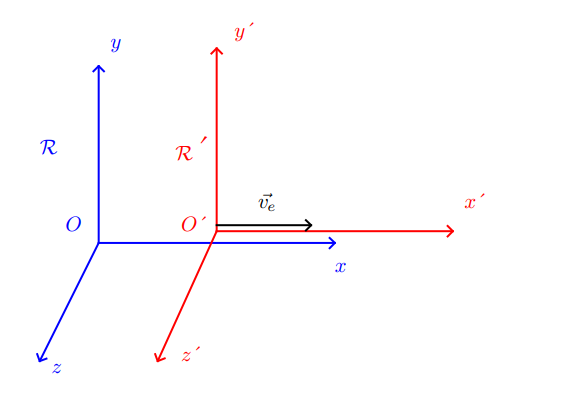
\includegraphics[width=.5\textwidth]{refgalileen.png}
% 	\caption{Référentiels en translation l'un par rapport à l'autre}
% \end{figure}

Dans ce contexte on définit une transformée pour passer des coordonnées d'un référentiel $\mathcal{R}$ à un autre $\mathcal{R}'$. On prend ces deux référentiels tels que à $t=0$, ils sont confondus, les horloges sont synchronisées. $t>0$ $\vec{v}(O') = v_e\vec{e_x}$. On peut alors décrire la position d'un point M par rapport au référentiel $\mathcal{R}$ grâce à \textbf{la transformée de Galilée}:


\begin{equation}
	\left\{\begin{array}{rcl}
		x(t) &=& x'+v_e t\\
		y(t) &=& y'\\
		z(t) &=& z'\\
		t &=& t'
	\end{array}\right.
\end{equation}

\textbf{Resultat:Loi de composition des vitesses}
	\begin{equation}
		v = v'+v_e
	\end{equation}


\subsection*{1.2. Qu'en est-il de l'électromagnétisme ?}
Les équations de Maxwell prédisent l'existence d'ondes se propageant à la vitesse $c$ a priori dans un référentiel privilégié (celui où sont définies les équations de Maxwell).

\begin{equation}
	\Delta E = \dfrac{1}{c^2}\dfrac{\partial^2 E}{\partial t^2} \text{ avec } c=\dfrac{1}{\sqrt{\epsilon_0\mu_0}}.
\end{equation}

On peut se demander quel est ce référentiel où des ondes peuvent se propager à une vitesse constante $c=3.0\cdot10^8~\rm m\cdot s^{-1}$. Si la vitesse de la lumière est définie dans un référentiel particulier et si elle obéit à la loi de composition des vitesses, on doit pouvoir mesurer une variation de la vitesse dans un autre référentiel. C'est ce que Michelson et Morley ont essayé de faire. 

\section*{2. Expérience de Michelson et Morley}

\textbf{Objectif:} Mesurer la variatio de la célérité de la lumière et vérifier que a lumière suit la loi de composition des vitesses.

\subsection*{2.1. Dispositif}

L'idée de Michelson et Morley est de se placer dans un référentiel qui se déplace par rapport au référentiel absolu dans lequel $c$ est définie. La planète Terre est en orbite quasi-circulaire de rayon $r=1.5\cdot 10^{11}~\rm m$ autour du soleil avec une période de $T = 365~\text{jours} = 3.15\cdot 10^{7}~ \rm s$. Ce qui donne une vitesse de la Terre autour du soleil de $v=3.0\cdot 10^4~\rm m\cdot s^{-1}$.

S'il existe un référentiel absolu pour la lumière on devrait pouvoir mesurer la variation de vitesse grâce à un dispositif suffisamment précis. Michelson construit un interféromètre dont l'idée est de faire interférer deux rayons lumineux ayant parcourus deux chemins différents .

\begin{center}
	\textbf{Bien décrire le dispositif expérimental sur transparents} (parcours des rayons, lame séparatrice, miroirs, détecteur)
\end{center}

% \begin{figure}[ht]
% 	\centering
% 	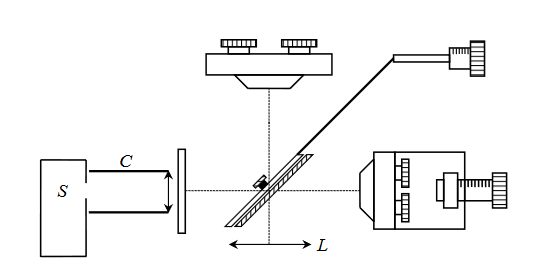
\includegraphics[width = .5\textwidth]{Michelson.png}
% 	\caption{Schéma de l'interféromètre de Michelson (\textit{Pérez, Relativité})}
% \end{figure}

L'éclairement sur le détecteur \textbf{P} dépend de $\Delta t$ le décalage temporel entre les rayons pour arriver sur le détecteur depuis la source. Les interférences dépendent de la phase : 

\begin{equation}
	\phi = 2\pi\nu\Delta t.
\end{equation}

\subsection*{2.2. Expression de la différence de phase}

On souhaite exprimer le retard d'un rayon par rapport à l'autre:

\begin{equation}
	\Delta t = T_{\parallel}-T_{\perp}
\end{equation}

On se place dans le référentiel lié au soleil et on suppose la Terre en translation rectiligne uniforme autour du soleil. L'interféromètre est placé sur Terre et se déplace à la vitesse $v_e = 3\cdot 10^4 ~\rm m\cdot s^{-1}$ par rapport au soleil. 

\subsubsection*{2.2.1. Chemin perpendiculaire:}

% \begin{figure}[ht]
% 	\centering
% 	\includegraphics[width=.5\textwidth]{schematrajetperp.png}
% 	\caption{Schéma chemin n$^\circ 1$}
% 	% \label{fig:chemin1}
% \end{figure}

On applique le théorême de Pythagore au triangle rectangle (ABC) de la figure 3:
\begin{equation}
	(ct)^2=L^2+(v_et)^2 \nonumber
\end{equation}

On factorise par le temps, le rayon issu de la lame séparatrice met un temps $t$ pour aller jusqu'au miroir $M_2$: 
\begin{equation}
	t=\dfrac{L}{c}\dfrac{1}{\sqrt{1-\left(\dfrac{v_e}{c}\right)^2}}. \nonumber
\end{equation}

En comptant le retour on en déduit $T_\perp$:
\begin{equation}
	T_\perp=2t=\dfrac{2L}{c}\dfrac{1}{\sqrt{1-\left(\dfrac{v_e}{c}\right)^2}}
\end{equation}

\subsubsection*{2.2.2. Chemin longitudinal:}
% \begin{figure}[ht]
% 	\centering
% 	\includegraphics[width=.4\textwidth]{schematrajetlongitudinal.png}
% 	\caption{Schéma chemin n$^\circ 1$}
% 	% \label{fig:chemin2}
% \end{figure}

Dans ce cas le dispositif se déplace parallèlement au rayon lumineux dont le rayon doit rattraper le miroir qui s'éloigne en même temps que le rayon avance tandis que le retour sera plus rapide car la lame semi-réfléchissante se rapproche du rayon réfléchi.

\begin{equation}
	\text{À l'aller : } t_{1} = \dfrac{L}{c+v_e}~\text{ au retour } t_2=\dfrac{L}{c-v_e}.\nonumber
\end{equation}

On en déduit $T_\parallel$:
\begin{equation}
	T_\parallel=\dfrac{2L}{c}\dfrac{1}{1-\left(\dfrac{v_e}{c}\right)^2}.
\end{equation}

Enfin, on peut exprimer le décalage temporel entre les rayons passant dans chaque bras de l'interféromètre: 

\begin{equation}
	\Delta t = T_\parallel - T_\perp = \dfrac{2L}{c}\left[\dfrac{1}{1-\left(\dfrac{v_e}{c}\right)^2}-\dfrac{1}{\sqrt{1-\left(\dfrac{v_e}{c}\right)^2}}\right]
\end{equation}

On fait le développement au premier ordre des fractions avec $v_e/c <<1$, en simplifiant les expressions il vient: 

\begin{equation}
	\Delta t = \dfrac{L}{c}\left(\dfrac{v_e}{c}\right)^2
\end{equation}

\subsection*{2.3. Résultats}

Par conséquent on peut prévoir le déphasage qu'engendre un tel décalage temporel: 
\begin{equation}
	\phi = 2\pi\dfrac{L\nu}{c}\left(\dfrac{v_e}{c}\right)^2 = 2\pi\dfrac{L}{\lambda}\left(\dfrac{v_e}{c}\right)^2.
\end{equation}

En prenant en compte les améliorations apportées par Morley à l'interféromètre de Michelson. Les bras du Michelson mesurent en comptant les réflexions $L=11~\rm m$, la longueur d'onde du Laser est de $\lambda=550~\rm m$. On trouc un déphasage 
\begin{equation}
	\dfrac{\phi}{2\pi} = 0.2
\end{equation}

Cela devrait être suffisant pour détecter un déplacement des franges de la figure d'interférence. Cependant le déplacement observé en pratique est nettement plus faible. Michelson et Morley observent un déplacement maximum de l'ordre de 0.02, en moyenne de 0.01.

% \begin{figure}[ht]
% 	\centering
% 	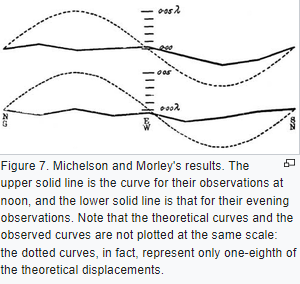
\includegraphics[width=.5\textwidth]{resultsMichelsonMorley.png}            \caption{Résultats obtenus par Michelson et Morley (\textit{Wikipedia})}
% 	% \label{fig:resMM}
% \end{figure}

\begin{definition}{Conclusion}
	On en conclut que l'on ne peut pas vérifier l'hypothèse suivant laquelle $c$ suit la loi de composition des vitesses. La mesure de la vitesse de la lumière semble indépendante du mouvement de la Terre par rapport au soleil. On peut alors prendre deux positions: 
	\begin{enumerate}
		\item Essayer de réparer la théorie du référentiel dans lequel sont définies les équations de Maxwell. 
		\item Plus courageux, admettre que $c$ est un invariant qui n'obéit pas aux lois de la cinématique galiléenne. Cela implique une nouvelle cinématique, c'est ce qu'a proposé Einstein en 1805 et que nous allons voir dans la partie suivante.
	\end{enumerate}
\end{definition}

\section*{3. Fondements de la relativité restreinte}

\subsection*{3.1. Postulats}

\begin{enumerate}
	\item Invariance des lois de la Physique
	
Toutes les lois de la physique sont invariantes par changement de référentiel galiléen. C'est à dire que les même lois se traduisent par des relations qui gardent la même structure au passage à un autre référentiel.
	\item Invariance de la vitesse de la lumière
	
Les équations de Maxwell sont invariantes par changement de référentiel. La célérité de la lumière est un invariant relativiste par changement de référentiel.

\begin{definition}{Définition - Célérité de la lumière}
	\begin{equation}
		c = \dfrac{1}{\sqrt{\epsilon_0\mu_0}}=3.0\cdot 10^8~\rm m\dot s^{-1}.
	\end{equation}
\end{definition}

À ce stade on peut revenir sur l'expérience de Michelson et Morley, car si $c=\rm constante$ alors il $\Delta t = 0$.

	\item Transformation de Lorentz poincaré
\begin{definition}{Définition - Transformée de Lorenz}
	\begin{equation}
		\left\{\begin{array}{rcl}
			ct &=& \gamma\left(ct'+\beta x'\right)\\
			x &=& \gamma\left(x'+\beta ct'\right)\\
			y &=& y'\\
			z &=& z'
		\end{array}\right.
	\end{equation}
\end{definition}	
\end{enumerate}

\subsection*{3.2. L'espace et le temps}


\subsubsection*{3.2.1. Notions d'évènements}

Le temps n'est plus un invariant, on ne peut plus le séparer des coordonnées spatiales. Il faut décrire les expériences en termes d'évènements : "Il s'est passé quelque chose quelque part" comme par exemple allumage d'une lampe sur l'ISS. Les évènements sont indépendants du référentiel.

\subsubsection*{3.2.2. Représentation spatiale}

% \begin{figure}[ht]
% 	\centering
% 	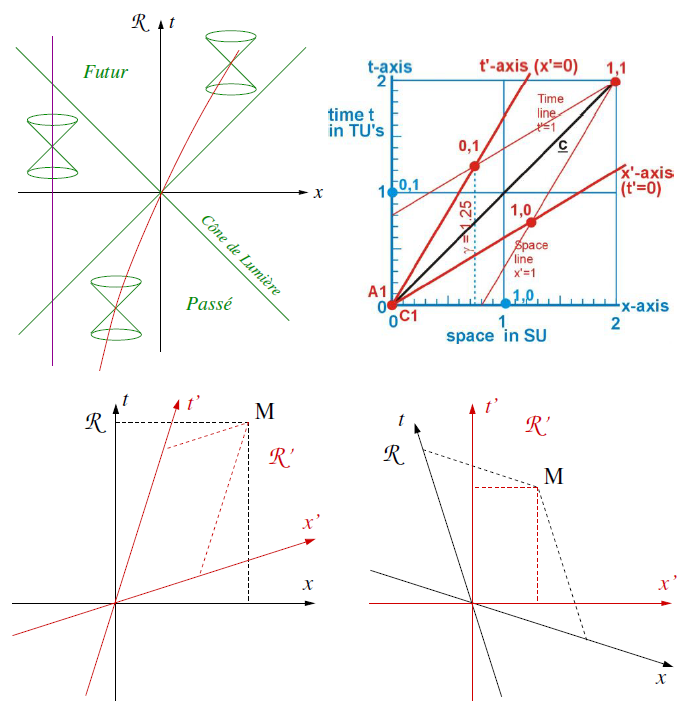
\includegraphics[width=.5\textwidth]{Minkowski.png}
% 	\caption{Diagramme espace-temps (diagramme de Minkowski)}
% \end{figure}

Deux évènements sont séparés par ce que l'on appelle l'intervalle, notée $\Delta s$. 

\begin{equation}
	\Delta s = c^2t^2-x^2-y^2-z^2
\end{equation}

L'intervalle est un invariant par changement de référentiel: $\Delta s = \Delta s'$. (commenter les valeurs de $\Delta s$ sur le graphique)

\subsection*{3.3. Conséquences de la relativité restreinte. Application au paradoxe du train et du tunnel (exercice)}

\textbf{Énoncé:} On a un train de longueur $L'$ mesuré dans $\mathcal{R}'$ (référentiel lié au train) animé d'une vitesse $\vec{v}=0.54c\vec{e}_x$ par rapport au référentiel $\mathcal{R}$ lié au tunnel (de longueur $L$ dans $\mathcal{R}'$). Le train rentre dans le tunnel rectiligne lors de l'évènement $A_1$. On prendra cet évènement comme origine spatiale et temporelle pour cet exercice où les deux référentiels sont confondus. On définit les évènements suivants:

\begin{itemize}
	\item $A_1$: l'avant du train rentre dans le tunnel : $\begin{pmatrix}
		x_{A_1}\\
		ct_{A_1}
	\end{pmatrix}_{\mathcal{R}} = \begin{pmatrix}
		0\\
		0
	\end{pmatrix}=\begin{pmatrix}
		x'_{A_1}\\
		ct'_{A_1}
	\end{pmatrix}_{\mathcal{R}'} $

	\item $A_2$: l'arrière du train entre dans le tunnel : $\begin{pmatrix}
		x_{A_2}\\
		ct_{A_2}
	\end{pmatrix}_{\mathcal{R}}$

	\item $B_1$: l'avant du train sort du tunnel : $\begin{pmatrix}
		x_{B_1}\\
		ct_{B_1}
	\end{pmatrix}_{\mathcal{R}}$

	\item $B_2$: l'arrière du train sort du tunnel : $\begin{pmatrix}
		x_{B_2}\\
		ct_{B_2}
	\end{pmatrix}_{\mathcal{R}} $
\end{itemize}

% \begin{figure}[ht]
% 	\centering
% 	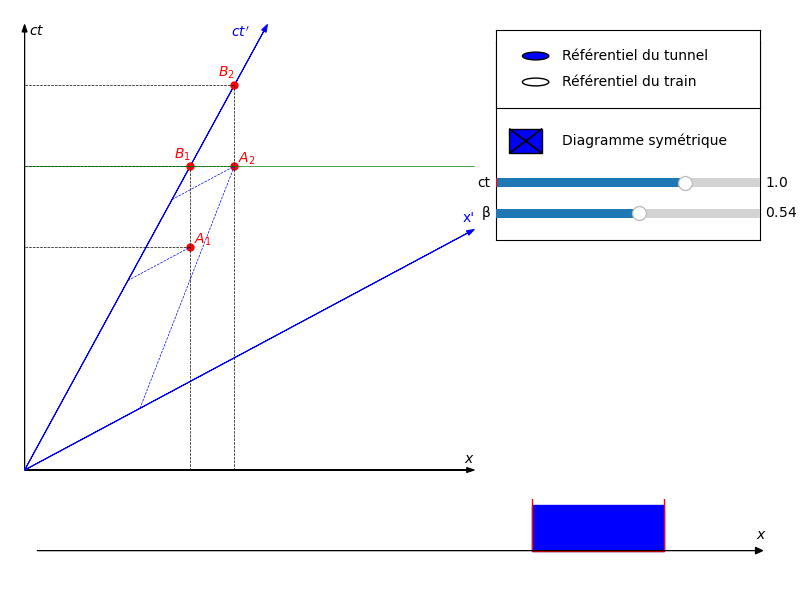
\includegraphics[width = .5\textwidth]{TrainEinstein.png}
% 	\caption{Simulation du paradoxe du train à discuter avec les calculs suivants}
% \end{figure}

\subsubsection*{3.3.1. Relativitié simultanéité}

Si nous disons que le train à 7h précise du matin sera complètement dans le tunnel, \textit{i.e.} $ct_{A_2}=ct_{B_1}$ dans le référentiel de l'observateur lié au tunnel. Dans le cadre de la relativité galiléenne où le temps est un invariant, dans le référentiel $\mathcal{R}'$ du train on aura aussi $t = t'$.

En cinématique relativiste ce n'est pas vrai: 

\begin{equation}
	\begin{array}{rcl}
	ct'_{A_2}-ct'_{B1} &= \gamma\left(ct_{A_2}-\beta x_{A_2}\right)-\gamma\left(ct_{B_1}-\beta x_{B_1}\right)\\
	&= \gamma\left(ct_{A_2}-ct_{B_1}\right)-\gamma\beta\left(x_{A_2}-x_{B_1}\right)\\
	&= \gamma\beta L
	\end{array}
\end{equation}

Les deux évènements simultanés dans $\mathcal{R}$ ne le sont pas dans $\mathcal{R}'$. (Le montrer à l'aide de la simulation).

\subsubsection*{3.3.2. Relativitié simultanéité}

Dans $\mathcal{R}'$ le trains mesure une longueur $L'$ c'est la longueur propre du train dans son référentiel propre. On peut mesurer sa taille dans le référentiel du tunnel. 

\begin{equation}
	\begin{array}{rcl}
		L'  &= x'_{A_2}-x'_{B_1}\\
            &= \gamma(x_{A_2}-\beta ct_{A_2})-\gamma(x_{B_1}-\beta ct_{B_1})\\
		    &= \gamma(x_{A_2}-x_{A_1})-\beta\gamma(ct_{A_2}-ct_{B_1})\\
		L'&= \gamma L
	\end{array}
\end{equation}

On en déduit que la longueur du train dans $\mathcal{R}$ est plus petite que dans $\mathcal{R}'$ (Le montrer à l'aide de la simulation).

\subsubsection*{3.3.3. Dilatation du temps}

Pour deux évènements, on peut établir la relation entre le temps propre et le temps mesuré dans un autre référentiel à condition que $x'2=x'1$ comme par exmpe pour les évènements $A_1$ et $B_1$.

On calcule : 

\begin{equation}
	\begin{array}{rcl}
		ct_{B_1}-ct_{A_1} &=& \gamma(ct'_{B_1}-ct'_{A_1})\\
		T_{\rm impropre} &=& \gamma T_{\rm propre}.
	\end{array}
\end{equation}

\subsection*{3.4. Loi de composition des vitesses}

\begin{equation}
	\left\{\begin{array}{rcl}
		ct &=& \gamma\left(ct'+\beta x'\right)\\
		x &=& \gamma\left(x'+\beta ct'\right)\\
		y &=& y'
	\end{array}\right.\leftrightarrow \left\{\begin{array}{rcl}
		dt &=& \gamma\left(dt'+\dfrac{v_e}{c^2} dx'\right)\\
		dx &=& \gamma\left(dx'+v_e dt'\right)\\
		dy &=& dy'
	\end{array}\right. \nonumber
\end{equation}

On obtient les vitesses en dérivant les coordonnées spatiales par rapport au temps : 
\begin{equation}
	\left\{\begin{array}{rcl}
		v_x = \dfrac{dx}{dt} &=& \dfrac{v_x'+v_e}{1+v_e\dfrac{v_x'}{c^2}}\\
		v_y = \dfrac{dy}{dt} &=& \dfrac{v_y'}{\gamma(1+v_e\dfrac{v_x'}{c^2})}
	\end{array}\right.
\end{equation}

\section*{Conclusion}

Pour ce premier cours de relativité restreinte, nous avons établi les bases d'une nouvelle cinématique. Il faut maintenant établir une nouvelle dynamique. Ainsi dans un prochain cours nous mettrons en équation la dynamique relativiste, en particulier nous écrirons les quadrivecteurs énergie et impulsion pour une particule en mouvement.


\end{document}

%%
%% FIN DU DOCUMENT
%%
